\documentclass[tikz,border=4pt]{standalone}
\usepackage{mathptmx}
\usepackage{amsmath,amssymb}
\DeclareMathAlphabet{\mathcal}{OMS}{cmsy}{m}{n}
\usetikzlibrary{positioning,arrows.meta,calc,fit}
\definecolor{cA}{HTML}{4A6FA5}\definecolor{fA}{HTML}{EEF3FA}
\definecolor{cB}{HTML}{5E9E4F}\definecolor{fB}{HTML}{EFF7EA}
\definecolor{cC}{HTML}{D19A1E}\definecolor{fC}{HTML}{FFF6DD}
\definecolor{cD}{HTML}{D9763A}\definecolor{fD}{HTML}{FDEFE5}
\definecolor{cE}{HTML}{2E8B8B}\definecolor{fE}{HTML}{E6F4F4}
\definecolor{cF}{HTML}{6E52B5}\definecolor{fF}{HTML}{F0ECFA}
\definecolor{cG}{HTML}{C9483F}\definecolor{fG}{HTML}{FCEDEC}
\definecolor{cH}{HTML}{2F5E9E}\definecolor{fH}{HTML}{E9F0FA}
\definecolor{cI}{HTML}{6B6B6B}\definecolor{fI}{HTML}{F2F2F2}
\definecolor{mt}{HTML}{2F4A7A}
\tikzset{>={Stealth[length=5pt]},
 stage/.style 2 args={draw=#1,fill=#2,line width=0.8pt,rounded corners=3pt,minimum width=10.4cm,minimum height=1.12cm,inner sep=0pt},
 % ---------- icons, drawn in a 0.8 x 0.8 cm frame centred at origin ----------
 pics/shieldlock/.style={code={
   \draw[line width=0.9pt,#1] (0,0.38) .. controls (0.18,0.30) and (0.30,0.30) .. (0.34,0.28) -- (0.34,0.02) .. controls (0.34,-0.20) and (0.15,-0.32) .. (0,-0.40) .. controls (-0.15,-0.32) and (-0.34,-0.20) .. (-0.34,0.02) -- (-0.34,0.28) .. controls (-0.30,0.30) and (-0.18,0.30) .. (0,0.38) -- cycle;
   \draw[line width=0.9pt,#1] (-0.12,-0.16) rectangle (0.12,0.04);
   \draw[line width=0.9pt,#1] (-0.075,0.04) -- (-0.075,0.10) arc (180:0:0.075) -- (0.075,0.04);
   \fill[#1] (0,-0.06) circle (0.025);}},
 pics/docsearch/.style={code={
   \draw[line width=0.9pt,#1] (-0.34,-0.38) -- (-0.34,0.38) -- (0.12,0.38) -- (0.26,0.24) -- (0.26,-0.02);
   \draw[line width=0.9pt,#1] (-0.34,-0.38) -- (-0.02,-0.38);
   \draw[line width=0.9pt,#1] (0.12,0.38) -- (0.12,0.24) -- (0.26,0.24);
   \foreach \y in {0.16,0.04,-0.08} \draw[line width=0.8pt,#1] (-0.24,\y) -- (0.06,\y);
   \draw[line width=0.9pt,#1] (0.16,-0.22) circle (0.12);
   \draw[line width=1.3pt,#1,line cap=round] (0.245,-0.305) -- (0.36,-0.42);}},
 pics/hierarchy/.style={code={
   \draw[line width=0.9pt,#1] (-0.09,0.22) rectangle (0.09,0.40);
   \draw[line width=0.9pt,#1] (-0.38,-0.40) rectangle (-0.20,-0.22);
   \draw[line width=0.9pt,#1] (0.20,-0.40) rectangle (0.38,-0.22);
   \draw[line width=0.9pt,#1] (0,0.22) -- (0,0) -- (-0.29,0) -- (-0.29,-0.22) (0,0) -- (0.29,0) -- (0.29,-0.22);}},
 pics/circuit/.style={code={
   \draw[line width=0.9pt,#1] (-0.28,0.24) -- (0.28,0.24) (-0.28,-0.24) -- (0.28,-0.24) (-0.28,0) -- (-0.08,0) (0.08,0) -- (0.28,0);
   \foreach \y in {0.24,0,-0.24} {\draw[line width=0.9pt,#1,fill=white] (-0.34,\y) circle (0.055); \draw[line width=0.9pt,#1,fill=white] (0.34,\y) circle (0.055);}
   \fill[#1] (-0.10,0.24) circle (0.045); \draw[line width=0.9pt,#1] (-0.10,0.24) -- (-0.10,-0.20);
   \draw[line width=0.9pt,#1] (-0.10,-0.24) circle (0.045);
   \draw[line width=0.9pt,#1,fill=white] (-0.02,-0.08) rectangle (0.18,0.08);}},
 pics/chip/.style={code={
   \draw[line width=0.9pt,#1] (-0.26,-0.26) rectangle (0.26,0.26);
   \fill[#1] (-0.16,-0.16) rectangle (0.16,0.16);
   \foreach \t in {-0.16,-0.053,0.053,0.16} {\draw[line width=0.8pt,#1] (\t,0.26) -- (\t,0.38) (\t,-0.26) -- (\t,-0.38) (0.26,\t) -- (0.38,\t) (-0.26,\t) -- (-0.38,\t);}}},
 pics/bars/.style={code={
   \fill[#1] (-0.36,-0.34) rectangle (-0.22,-0.12);
   \fill[#1] (-0.16,-0.34) rectangle (-0.02,0.00);
   \fill[#1] (0.04,-0.34) rectangle (0.18,0.16);
   \fill[#1] (0.24,-0.34) rectangle (0.38,0.34);}},
 pics/gauge/.style={code={
   \draw[line width=0.9pt,#1] (-0.36,-0.14) arc (200:-20:0.383);
   \foreach \a in {180,135,90,45,0} \draw[line width=0.8pt,#1] (\a:0.28)++(0,0.0) -- (\a:0.36);
   \draw[line width=1.2pt,#1,line cap=round] (0,-0.02) -- (58:0.26);
   \fill[#1] (0,-0.02) circle (0.05);}},
 pics/shieldcheck/.style={code={
   \fill[#1] (0,0.38) .. controls (0.18,0.30) and (0.30,0.30) .. (0.34,0.28) -- (0.34,0.02) .. controls (0.34,-0.20) and (0.15,-0.32) .. (0,-0.40) .. controls (-0.15,-0.32) and (-0.34,-0.20) .. (-0.34,0.02) -- (-0.34,0.28) .. controls (-0.30,0.30) and (-0.18,0.30) .. (0,0.38) -- cycle;
   \draw[white,line width=1.6pt,line cap=round,line join=round] (-0.15,-0.01) -- (-0.03,-0.13) -- (0.17,0.11);}},
 pics/podium/.style={code={
   \draw[line width=0.9pt,#1] (-0.13,-0.38) rectangle (0.13,0.38);
   \draw[line width=0.9pt,#1] (-0.39,-0.38) rectangle (-0.13,0.10);
   \draw[line width=0.9pt,#1] (0.13,-0.38) rectangle (0.39,-0.10);
   \node[font=\scriptsize\bfseries,text=#1,inner sep=0] at (0,0.20) {1};
   \node[font=\scriptsize\bfseries,text=#1,inner sep=0] at (-0.26,-0.08) {2};
   \node[font=\scriptsize\bfseries,text=#1,inner sep=0] at (0.26,-0.22) {3};}}
}
\newcommand{\stage}[7]{% name, prev, colour, fill, icon, title, body
 \node[stage={#3}{#4},#2] (#1) {};
 \pic at ([xshift=0.62cm]#1.west) {#5=#3};
 \node[align=center,font=\footnotesize,text width=8.9cm] at ([xshift=0.5cm]#1.center) {{\small\textbf{#6}}\\[-0.5pt]#7};
}
\begin{document}
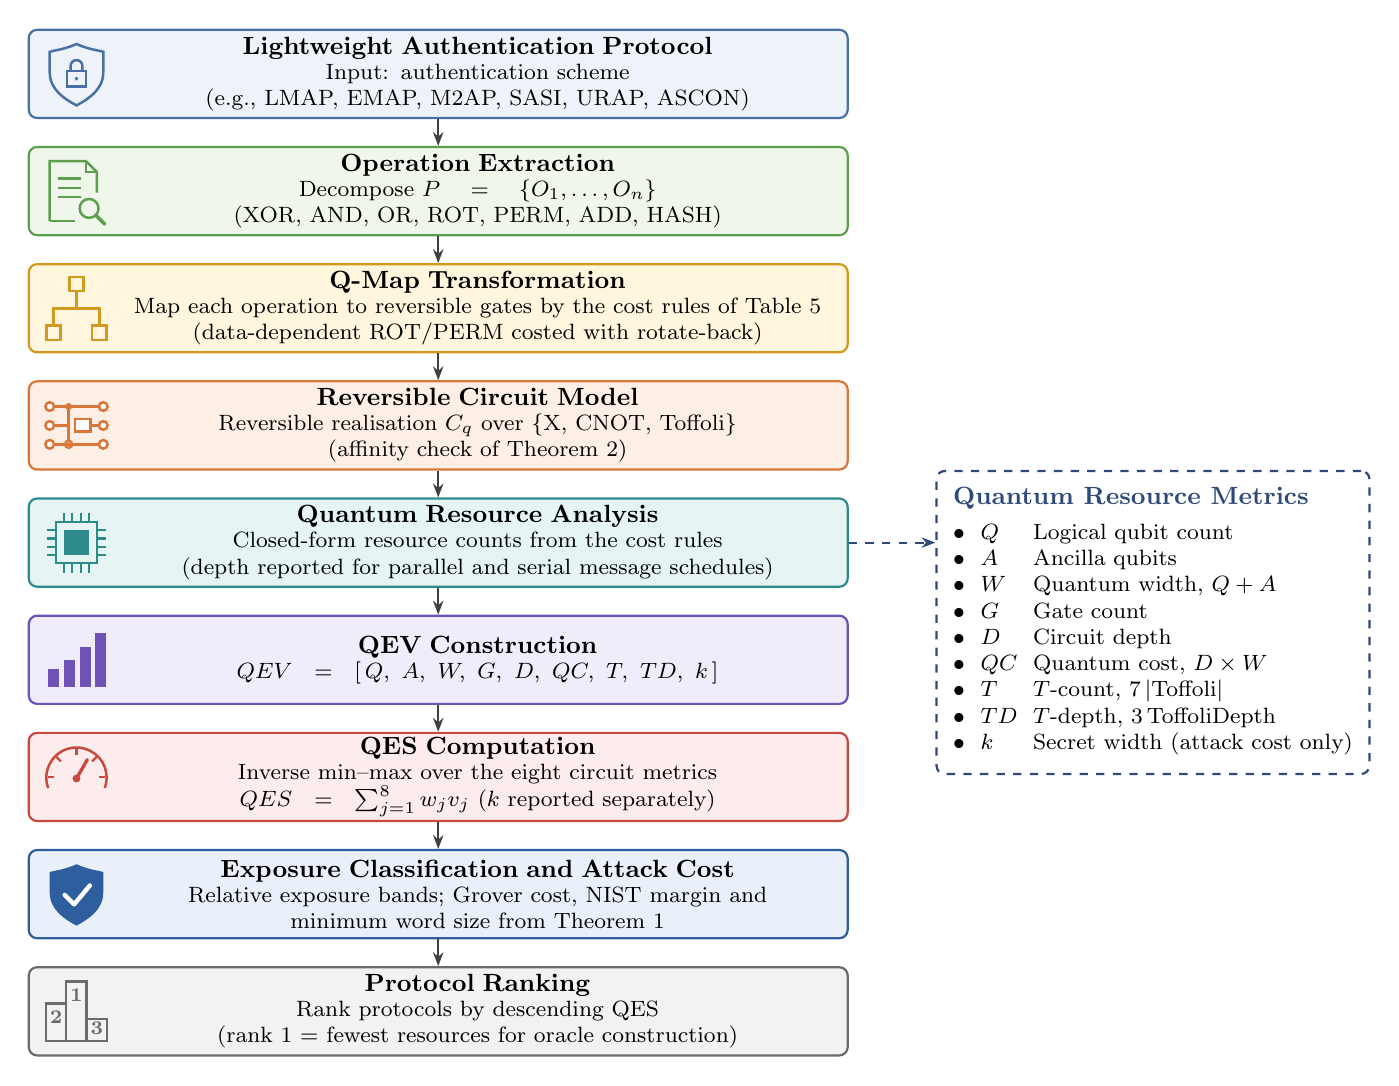
\begin{tikzpicture}
\stage{s1}{}{cA}{fA}{shieldlock}{Lightweight Authentication Protocol}{Input: authentication scheme\\(e.g., LMAP, EMAP, M2AP, SASI, URAP, ASCON)}
\stage{s2}{below=0.34cm of s1}{cB}{fB}{docsearch}{Operation Extraction}{Decompose $P=\{O_1,\dots,O_n\}$\\(XOR, AND, OR, ROT, PERM, ADD, HASH)}
\stage{s3}{below=0.34cm of s2}{cC}{fC}{hierarchy}{Q-Map Transformation}{Map each operation to reversible gates by the cost rules of Table 5\\(data-dependent ROT/PERM costed with rotate-back)}
\stage{s4}{below=0.34cm of s3}{cD}{fD}{circuit}{Reversible Circuit Model}{Reversible realisation $C_q$ over \{X, CNOT, Toffoli\}\\(affinity check of Theorem 2)}
\stage{s5}{below=0.34cm of s4}{cE}{fE}{chip}{Quantum Resource Analysis}{Closed-form resource counts from the cost rules\\(depth reported for parallel and serial message schedules)}
\stage{s6}{below=0.34cm of s5}{cF}{fF}{bars}{QEV Construction}{$QEV=[\,Q,\ A,\ W,\ G,\ D,\ QC,\ T,\ TD,\ k\,]$}
\stage{s7}{below=0.34cm of s6}{cG}{fG}{gauge}{QES Computation}{Inverse min--max over the eight circuit metrics\\$QES=\sum_{j=1}^{8} w_j v_j$ ($k$ reported separately)}
\stage{s8}{below=0.34cm of s7}{cH}{fH}{shieldcheck}{Exposure Classification and Attack Cost}{Relative exposure bands; Grover cost, NIST margin and\\minimum word size from Theorem 1}
\stage{s9}{below=0.34cm of s8}{cI}{fI}{podium}{Protocol Ranking}{Rank protocols by descending QES\\(rank 1 = fewest resources for oracle construction)}
\foreach \a/\b in {s1/s2,s2/s3,s3/s4,s4/s5,s5/s6,s6/s7,s7/s8,s8/s9}
  \draw[->,line width=0.8pt,black!75] (\a.south) -- (\b.north);
% metrics panel
\node[draw=mt,dashed,line width=0.8pt,rounded corners=3pt,anchor=north west,minimum width=4.9cm,inner sep=6pt,align=left,font=\footnotesize]
 (M) at ([xshift=1.1cm,yshift=0.35cm]s5.north east) {%
 {\small\textbf{\textcolor{mt}{Quantum Resource Metrics}}}\\[3pt]
 \begin{tabular}{@{}l@{\ \ }l@{\ \ }l@{}}
 $\bullet$ & $Q$ & Logical qubit count\\
 $\bullet$ & $A$ & Ancilla qubits\\
 $\bullet$ & $W$ & Quantum width, $Q+A$\\
 $\bullet$ & $G$ & Gate count\\
 $\bullet$ & $D$ & Circuit depth\\
 $\bullet$ & $QC$ & Quantum cost, $D\times W$\\
 $\bullet$ & $T$ & $T$-count, $7\,|\mathrm{Toffoli}|$\\
 $\bullet$ & $TD$ & $T$-depth, $3\,\mathrm{ToffoliDepth}$\\
 $\bullet$ & $k$ & Secret width (attack cost only)
 \end{tabular}};
\draw[->,dashed,line width=0.8pt,mt] (s5.east) -- (s5.east -| M.west);
\end{tikzpicture}
\end{document}
